\chapter{Negative Pion Cross Section Measurement}\label{ch:PionXS}
%{\raggedleft ``\emph{Y ella es flama que se eleva, Y es un p\'ajaro a volar} \par}
%{\raggedleft \emph{En la noche que se incendia, Estrella de oscuridad}"\par}
%{\raggedleft \emph{Que busca entre la tiniebla, La dulce hoguera del beso}"\par}
%{\raggedleft -- Lila Downs, Benediction And Dream,  2002-- \par}


\section{Raw Cross Section}\label{ch:PionXSRaw}
We measure the ($\pi^-$-Ar) cross section as a function of the kinetic energy in the two chosen data sets, the 60A and 100A negative runs. 
As will be clarified in \ref{ch:PionXSCorrections},  the corrections to the raw cross section depend on the beam conditions and need to proceed independently for the two data sets. Thus, we present here the two measurements separately.


As stated in section \ref{ch:XSRaw},  the raw cross section is given by the equation \label{eq:thinTargetXSSolved}
\begin{equation}
 \sigma_{TOT} (E_i)  = \frac{1}{n \delta X}\frac{N_{Interacting}(E_i)}{N_{Incident}(E_i)}.
\end{equation}

where $N_{Interacting}$  is the number of particles interacting in an argon slice at kinetic energy $E_i$, $N_{Incident}$ is number of particles incident  on the argon slice at   kinetic energy $E_i$,  $n$ is the density of the target centers  and $\delta X$ is the thickness of the argon slice.


Figure \ref{fig:InteractingRaw} shows the interacting histogram for the 60A dataset on the left and for the 100A dataset on the right. 
Figure \ref{fig:IncidentRaw} shows the incident histogram for the 60A dataset on the left and for the 100A dataset on the right. 
Figure \ref{fig:XSRaw} shows the raw cross section for the 60A dataset on the left and for the 100A dataset on the right. On all plots the same color scheme is used: the statistical uncertainty is shown in azure, while the systematic uncertainty is shown in blue. The calculation of the statistical unceratinty is laid out in section \ref{ch:StatUncertaintyXSRaw}, while the systematics on this \ref{ch:SysUncertaintyXSRaw}.

\begin{figure}[p]
\centering  
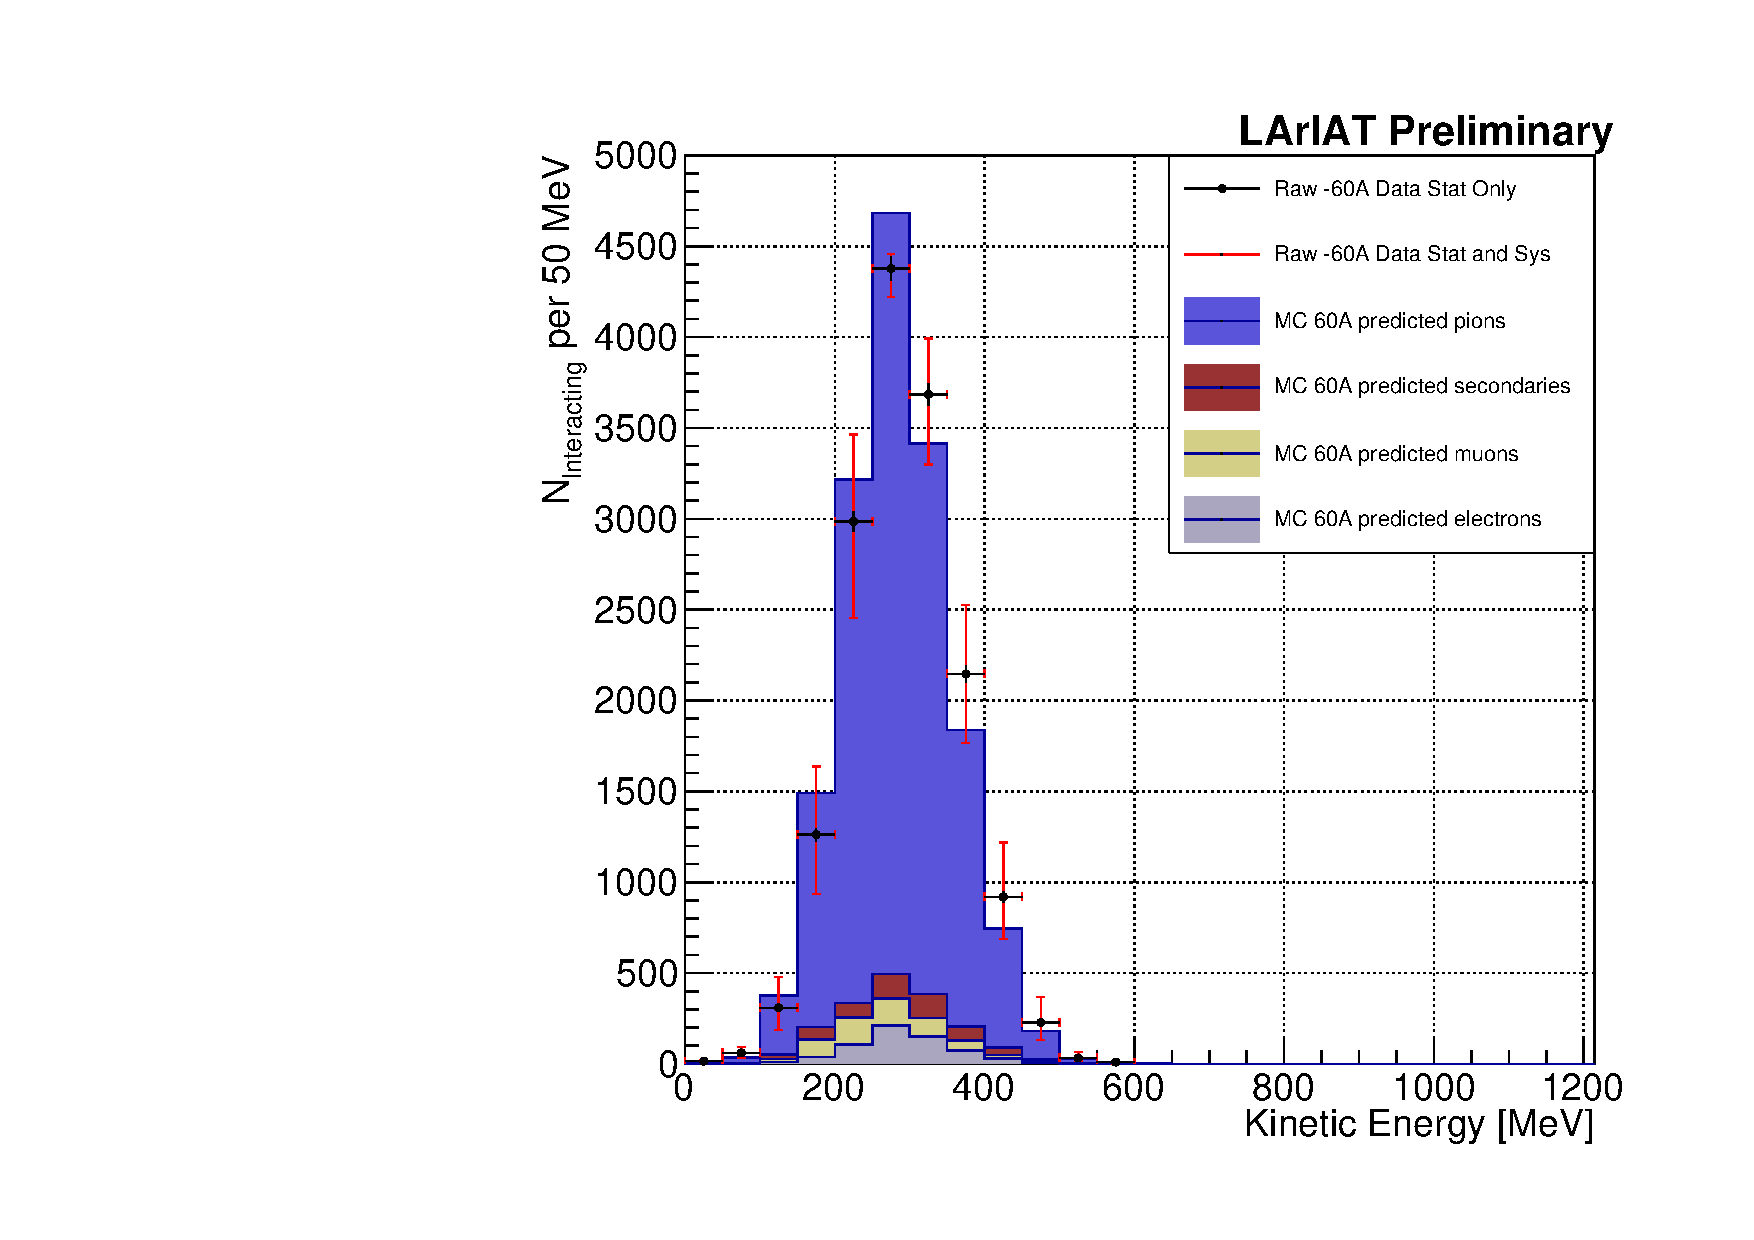
\includegraphics[width=0.48\textwidth]{Chapter-6/Images/Plots60A_MCData_Int_StatSyst.pdf}
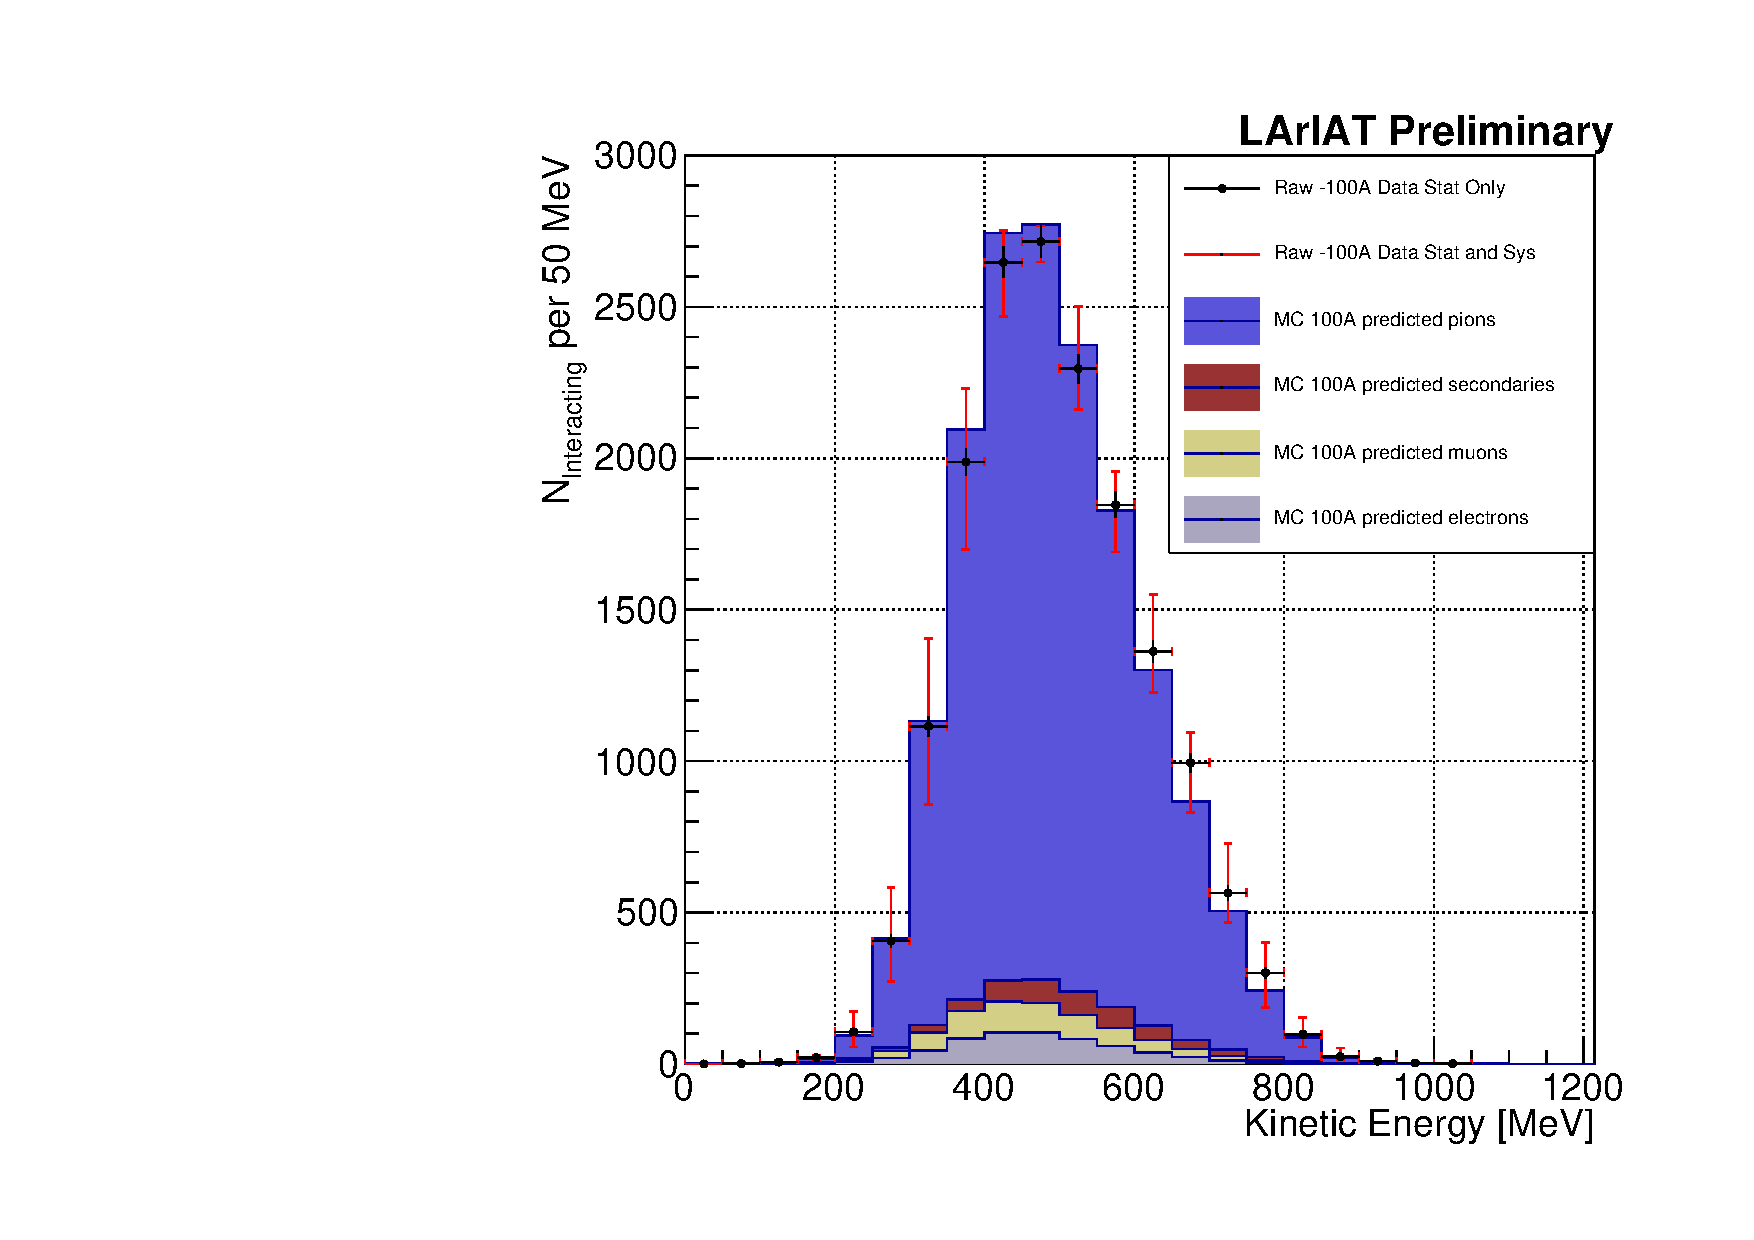
\includegraphics[width=0.48\textwidth]{Chapter-6/Images/Plots100A_MCData_Int_StatSyst.pdf}
\caption{Raw number of interacting pion candidates as a function of the reconstructed kinetic energy for the 60A runs (lef) and for the 100A runs (right). The statistical uncertainties are shown in azure, the systematic uncertainties in blue.}
\label{fig:InteractingRaw}
\end{figure}


\begin{figure}
\centering  
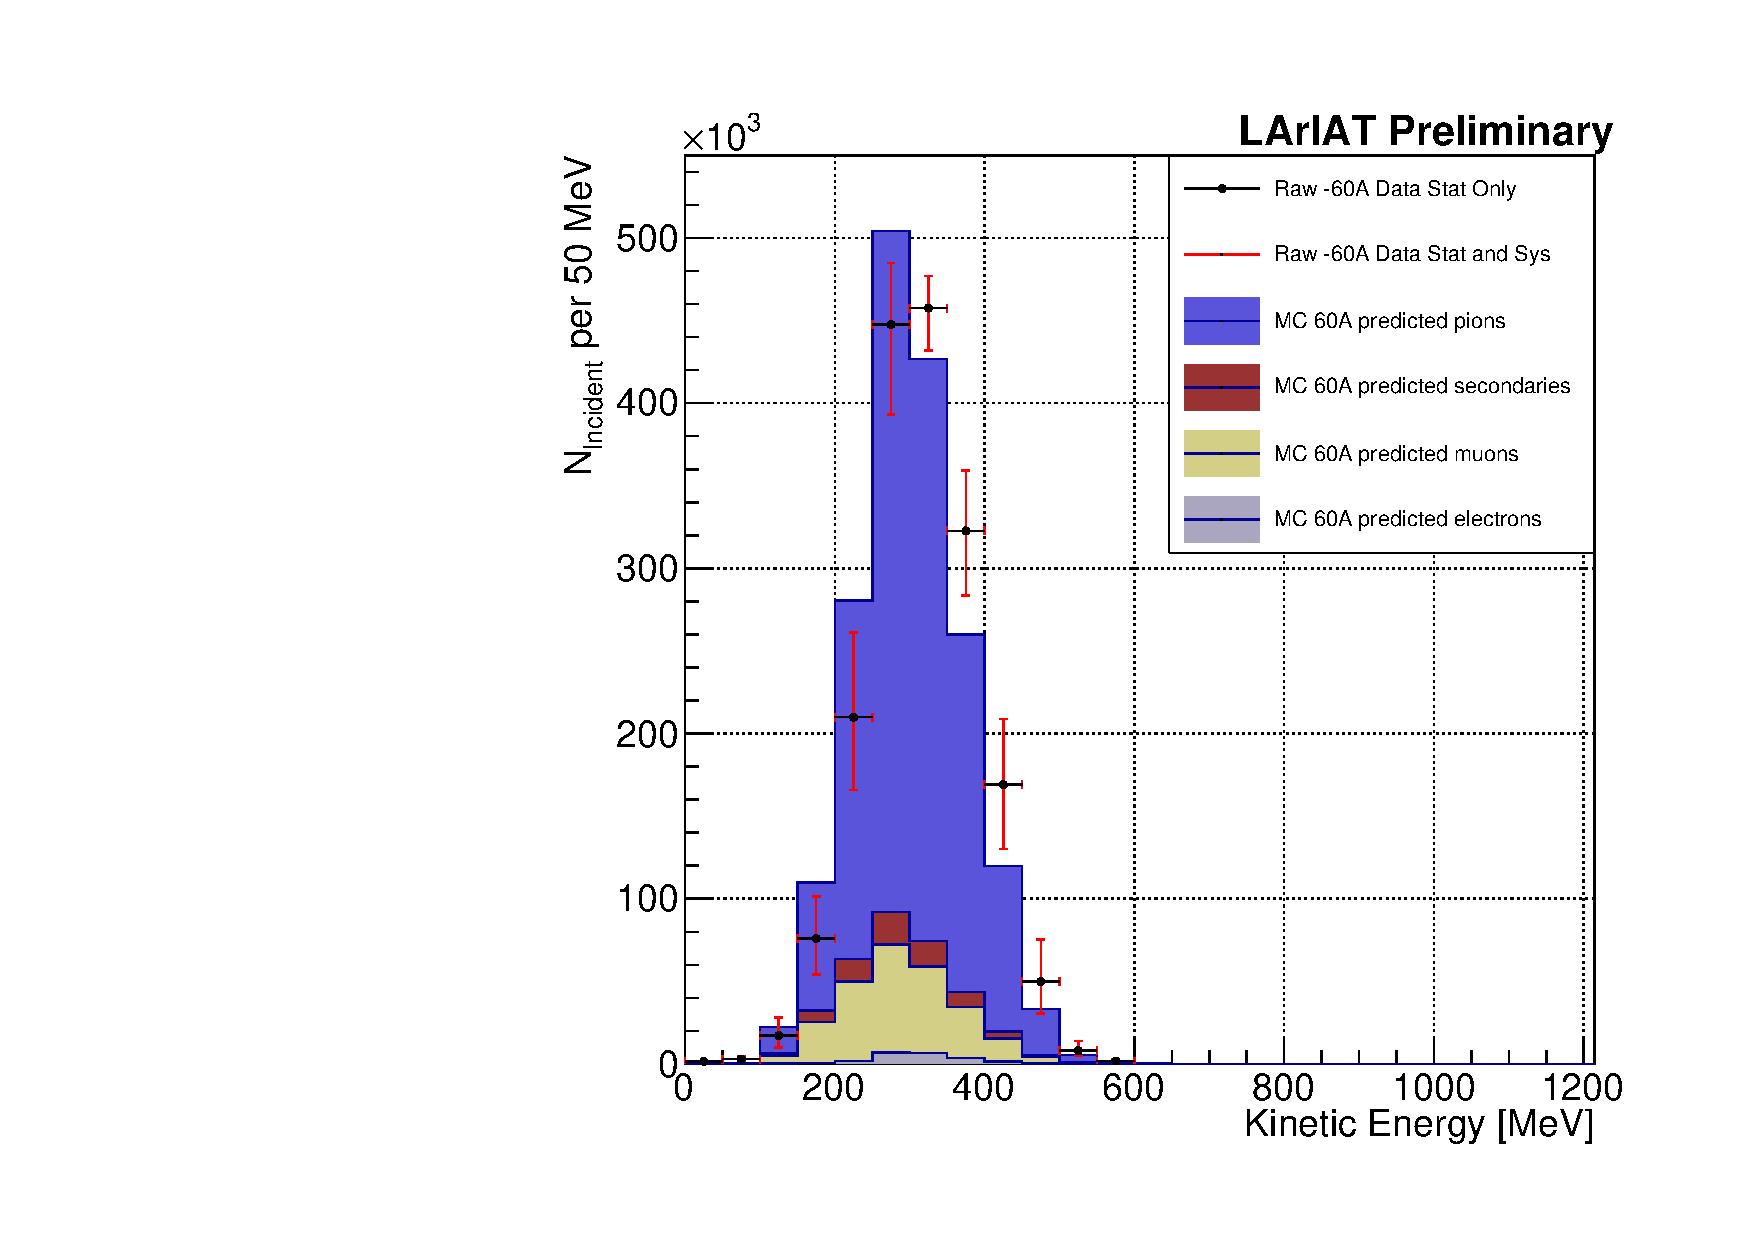
\includegraphics[width=0.48\textwidth]{Chapter-6/Images/Plots60A_MCData_Inc_StatSyst.pdf}
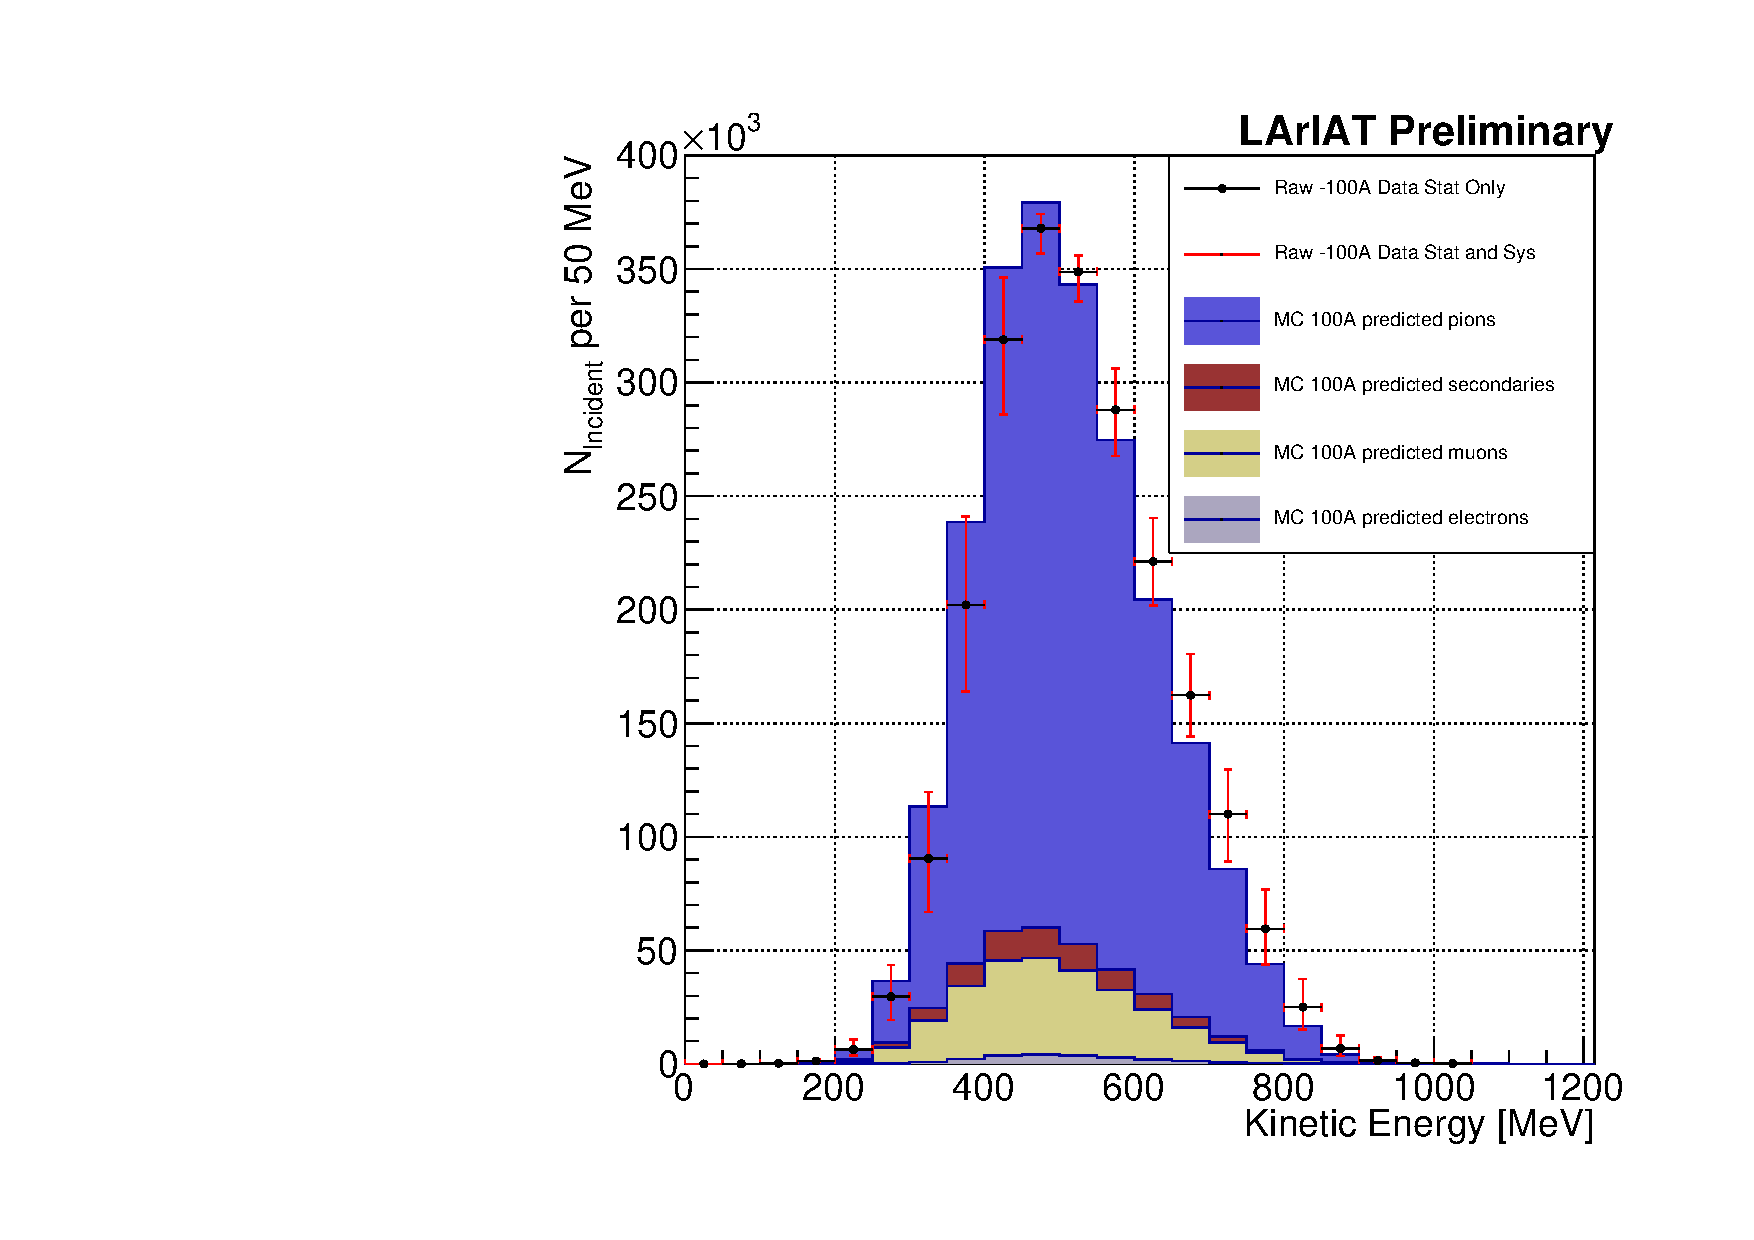
\includegraphics[width=0.48\textwidth]{Chapter-6/Images/Plots100A_MCData_Inc_StatSyst.pdf}
\caption{Raw number of incident pion candidates as a function of the reconstructed kinetic energy for the 60A runs (lef) and for the 100A runs (right). The statistical uncertainties are shown in azure, the systematic uncertainties in blue.}
\label{fig:IncidentRaw}
\end{figure}

\begin{figure}
\centering  
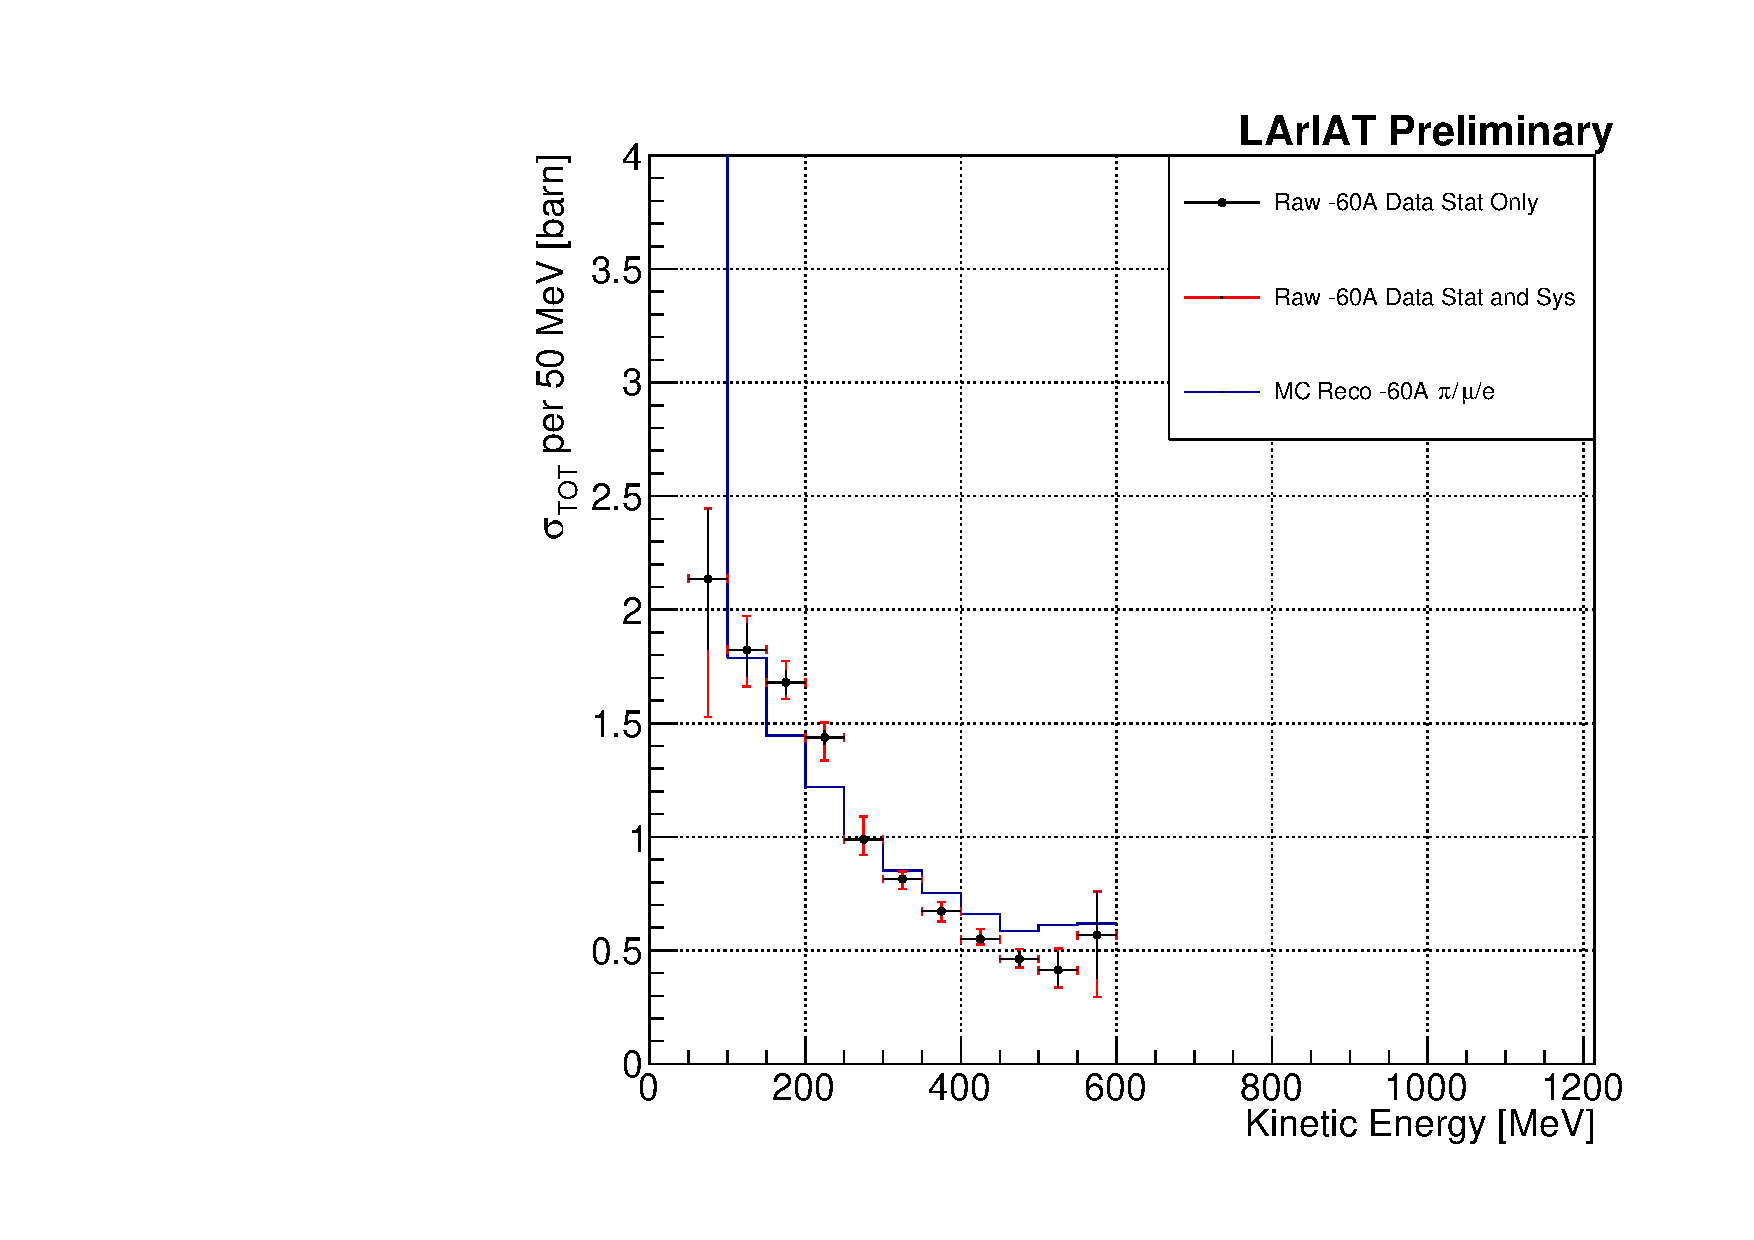
\includegraphics[width=0.48\textwidth]{Chapter-6/Images/Plots60A_MCData_XS_StatSyst.pdf}
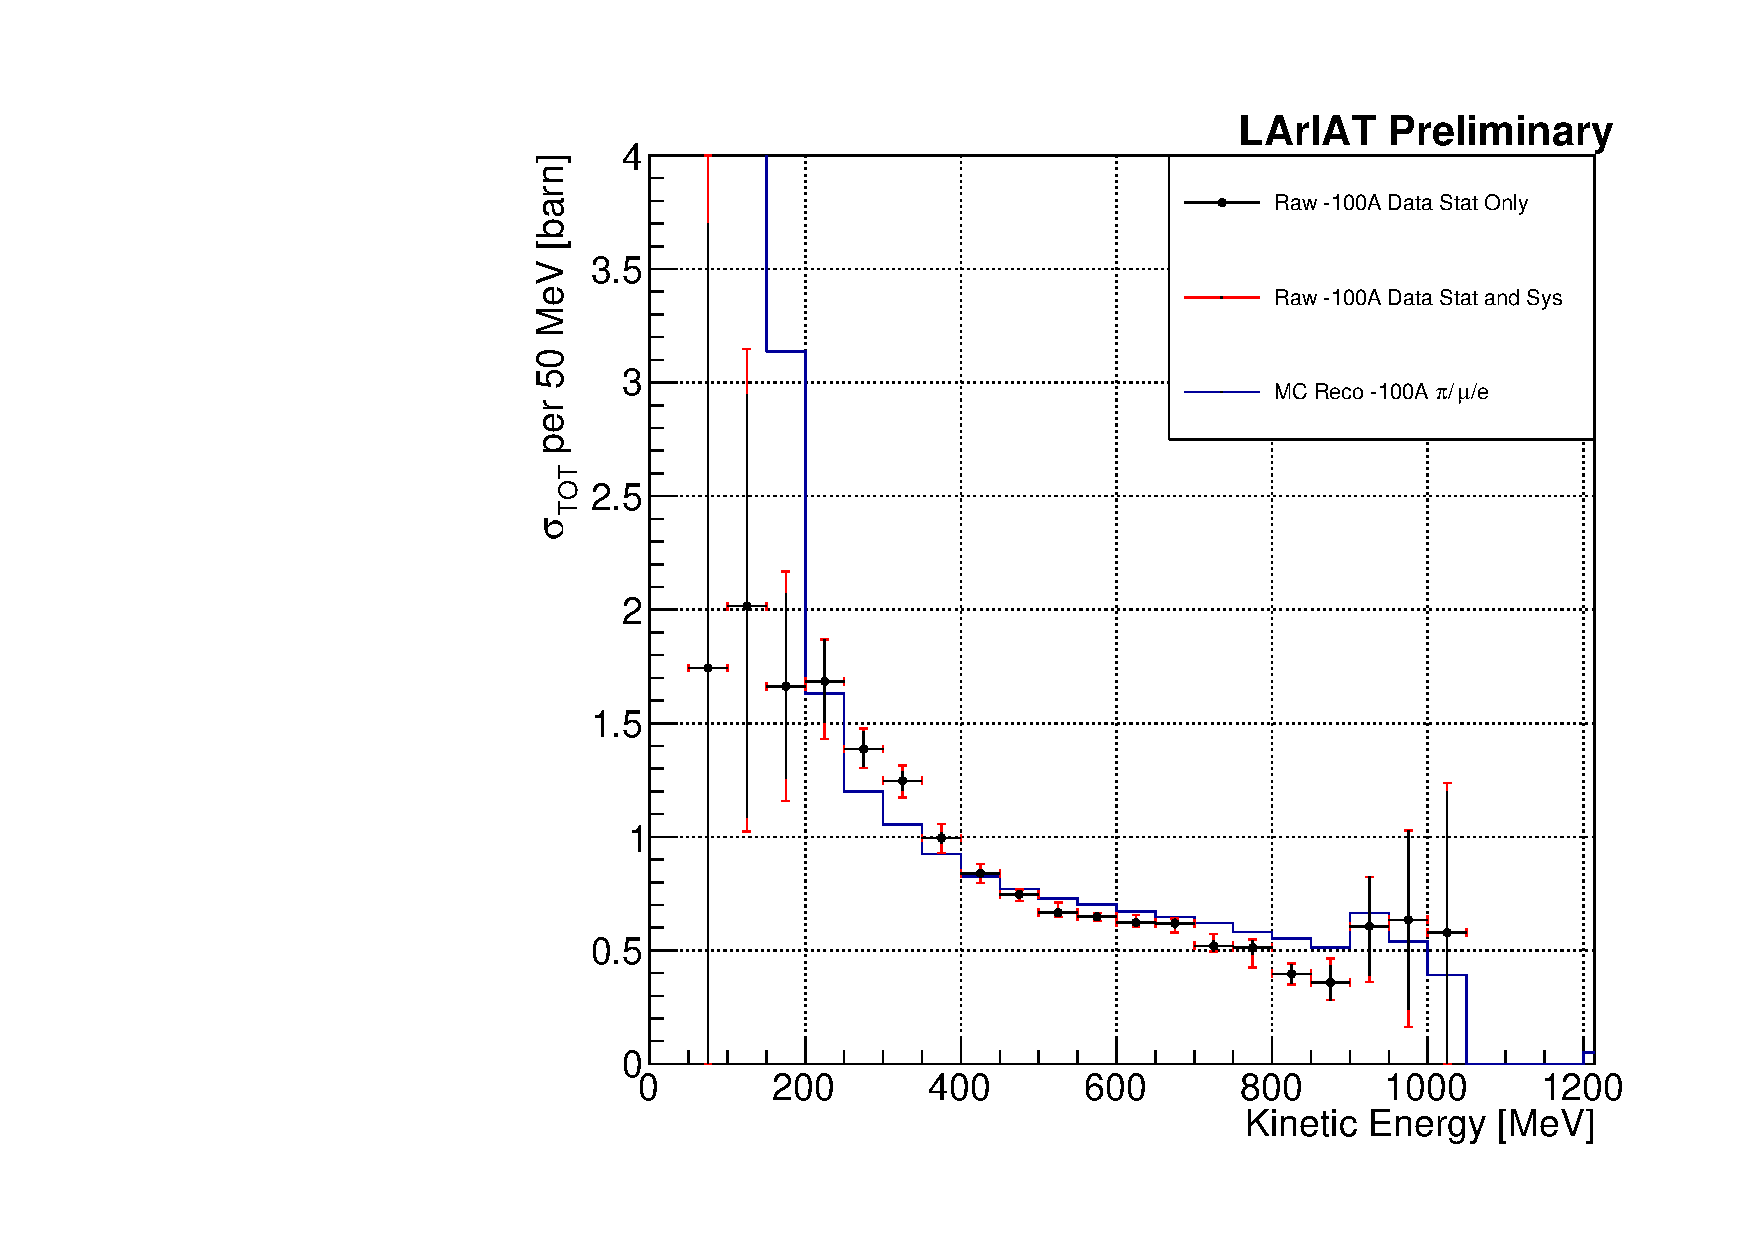
\includegraphics[width=0.48\textwidth]{Chapter-6/Images/Plots100A_MCData_XS_StatSyst.pdf}
\caption{Raw ($\pi^-$-Ar) total hadronic cross section for the 60A runs (lef) and for the 100A runs (right). The statistical uncertainties are shown in azure, the systematic uncertainties in blue.}
\label{fig:XSRaw}
\end{figure}


\subsection{Statistical Uncertainty}\label{ch:StatUncertaintyXSRaw}
The statistical uncertainty for each kinetic energy bin of the cross section plot is calculated by error propagation from the statistical uncertainty on $N_{Incident}$ and $N_{Interacting}$ correspondent bin.  Since the number of incident hadrons in each energy bin is given by a simple counting, we assume that $N_{Incident}$ is distributed as a poissonian with mean and variance equal to $N_{Incident}$ in each bin.  
On the other hand, $N_{Interacting}$ follows a binomial distribution: a particle in a given energy bin might or might not interact.  The variance for the binomial is given by  
\begin{equation}
\text{\textsf{Var[$N_{Incident}$]}} = \mathcal{N}P_{Interacting}(1-P_{Interacting});
\label{eq:binVar}
\end{equation}

since the interaction probability $P_{Interacting}$ is $\frac{ N_{Interacting}}{N_{Incident}}$ and the number of tries $\mathcal{N}$ is $N_{Incident}$, equation \ref{eq:binVar} translates into
\begin{equation}
\text{\textsf{Var[$N_{Incident}$]}} = N_{Incident}\frac{ N_{Interacting}}{N_{Incident}} (1-\frac{ N_{Interacting}}{N_{Incident}}) = N_{Interacting}(1-\frac{ N_{Interacting}}{N_{Incident}}). 
\end{equation}

$N_{Incident}$ and $N_{Interacting}$ are not independent.
The statistical uncertainty on the cross section is thus calculated as 
\begin{equation}
\delta\sigma_{tot}(E) = \sigma_{tot}(E) \Big(\frac{\delta N_{Interacting}}{N_{Interacting}}+\frac{\delta N_{Incident}}{N_{Incident}}\Big) 
\end{equation}
where:
\begin{eqnarray}
\delta N_{Incident} = \sqrt[]{N_{Incident}} \\
\delta N_{Interacting} = \sqrt[]{N_{Interacting}\Big(1-\frac{ N_{Interacting}}{N_{Incident}}\Big)}.
\end{eqnarray}



\subsection{Treatment of Systematics} \label{ch:SysUncertaintyXSRaw}
The only systematic effect considered in the measurement of the raw cross section results from the propagation of the uncertainty associate with the measurement of the kinetic energy at each slab.


\section{Corrections to the Raw Cross Section}\label{ch:PionXSCorrections}
\subsection{Treatment of Systematics}

